% !TEX TS-program = pdflatex
% Beamer pitch deck for Fan Wei (Duke)

\documentclass[aspectratio=169,11pt]{beamer}

% --------------------
% Theme / appearance
% --------------------
\usetheme{Madrid}
\usecolortheme{default}
\setbeamertemplate{navigation symbols}{}
\setbeamertemplate{footline}{%
  \leavevmode%
  \hbox{%
  \begin{beamercolorbox}[wd=.85\paperwidth,ht=2.5ex,dp=1ex,left]{author in head/foot}%
    \hspace{1.2em}\insertshorttitle
  \end{beamercolorbox}%
  \begin{beamercolorbox}[wd=.15\paperwidth,ht=2.5ex,dp=1ex,right]{date in head/foot}%
    \insertframenumber{} / \inserttotalframenumber\hspace{1.2em}
  \end{beamercolorbox}}%
  \vskip0pt%
}

% --------------------
% Packages
% --------------------
\usepackage{amsmath,amsfonts,amssymb,mathtools}
\usepackage{bbm}
\usepackage{booktabs}
\usepackage{graphicx}
\usepackage{tikz}
\usetikzlibrary{arrows.meta,positioning,calc,fit,shapes.geometric}
\usepackage{hyperref}

% --------------------
% Macros
% --------------------
\newcommand{\1}{\mathbbm{1}}
\newcommand{\E}{\mathbb{E}}
\newcommand{\Eb}{\widehat{\mathbb{E}}}
\newcommand{\Prb}{\mathbb{P}}
\newcommand{\cA}{\mathcal{A}}
\newcommand{\cH}{\mathcal{H}}
\newcommand{\cW}{\mathcal{W}}
\newcommand{\R}{\mathbb{R}}
\newcommand{\norm}[1]{\left\lVert#1\right\rVert}
\newcommand{\ip}[2]{\left\langle#1,#2\right\rangle}
\newcommand{\defeq}{\mathrel{\mathop:}=}
\newcommand{\polylog}{\mathrm{polylog}}

\title[Heavy-tailed COPF]{Heavy-tailed COPF: Heavy-Tailed, Dependency-Aware Certificates \& Control}
\date{Feb 2026}

\begin{document}

% --------------------
% Title
% --------------------
\begin{frame}
  \titlepage
  \vspace{-1.0em}

\end{frame}

% --------------------
% Agenda
% --------------------
\begin{frame}{Abstract}

    \small COPF makes \emph{deployment-stable counterfactual fairness} identifiable in online link recommendation; \newline
    I want to extend COPF to a theory-first paper where \textbf{(A)} fairness certificates hold under \textbf{heavy-tailed} residuals and \textbf{dependent graph data}, \textbf{(B)} the online controller converges without gradient clipping, and \textbf{(C)} the key dependence parameters (\(\kappa,\tau_{\mathrm{mix}}\)) become \emph{theorems} under a dynamic random-graph model.

\end{frame}

\begin{frame}{Agenda}
\begin{enumerate}
  \item Why COPF: fairness in performative, evolving graphs
  \item COPF pipeline: logging \(\to\) GA-DR \(\to\) Residual-OI \(\to\) control
  \item Where current theory is brittle: bounded residuals / clipping assumptions
  \item The new theory direction: heavy tails + dependence
  \item Three tasks
  \item \textbf{What I need from you}: concrete math tasks
\end{enumerate}
\end{frame}

% --------------------
% Motivation: performative fairness
% --------------------
\begin{frame}{Motivation: fairness drifts when recommendations change the graph}
\begin{columns}[T]
\begin{column}{0.55\textwidth}
\small
\begin{itemize}
  \item In link recommendation (``who to follow'' / ``what to connect''), the platform \textbf{chooses exposure}.
  \item Exposure changes what edges can form \(\Rightarrow\) the graph evolves \emph{because of the policy}.\newline
  \item Fairness computed on logged outcomes can be misleading (selection effects).
  \item We want \textbf{deployment-stable} fairness: comparable across different deployed policies.
\end{itemize}
\end{column}
\begin{column}{0.45\textwidth}
\begin{block}{Key idea}
\small Define fairness on \textbf{exposure counterfactuals}: for each candidate edge, compare what would happen if it were \emph{shown} vs \emph{not shown}, then compare across groups.
\end{block}
\begin{block}{Challenge}
\small We only see outcomes under the deployed policy, and graph data are dependent (temporal + network interference).
\end{block}
\end{column}
\end{columns}
\end{frame}

% --------------------
% COPF at a glance
% --------------------
\begin{frame}{COPF in one picture}
\begin{figure}
    \centering
    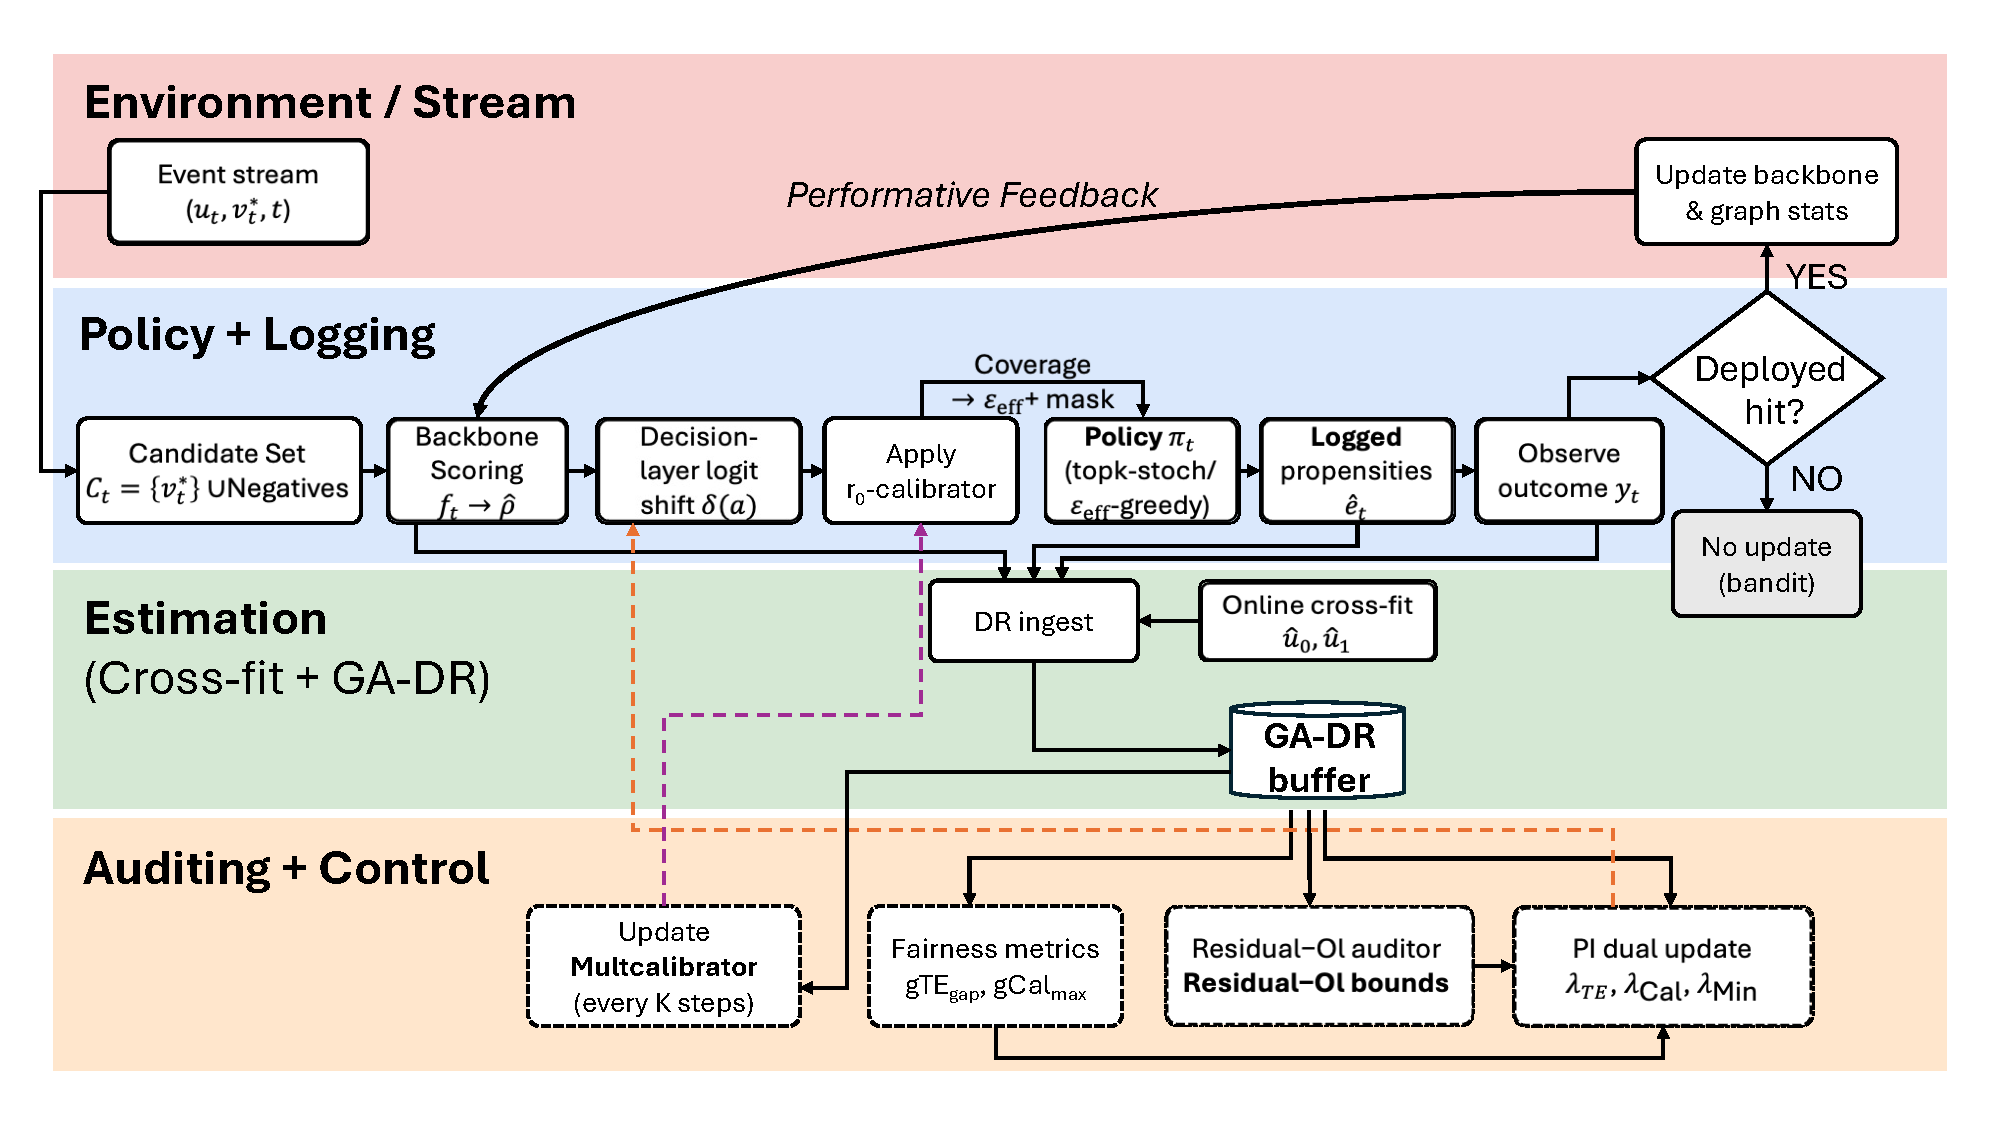
\includegraphics[width=0.9\linewidth]{Diagram.pdf}

\end{figure}
\end{frame}

% --------------------
% Problem definition details
% --------------------
\begin{frame}{Problem definition (what is observed vs counterfactual)}
\small
At each round $t$:
\begin{itemize}
  \item We build a context $W_t(u_t,v)$ from features and local graph summaries computed from $G_{\le t}$.
  \item Exposure policy selects a slate $D_t$ of size $K$ and we log per-candidate marginal propensity $\hat e_t(v)$.
\end{itemize}
\vspace{0.4em}
\begin{block}{Potential outcomes (counterfactuals)}
\small
For each candidate edge $(u_t,v)$ define
\[
Y_t^{(1)}(u_t,v)\in\{0,1\} \quad\text{(if exposed)}, \qquad
Y_t^{(0)}(u_t,v)\in\{0,1\} \quad\text{(if not exposed)}.
\]
Observed outcome:
\[
Y_t(u_t,v)=D_t(v)\,Y_t^{(1)}(u_t,v) + (1-D_t(v))\,Y_t^{(0)}(u_t,v).
\]
\end{block}
\end{frame}

\begin{frame}{What fairness means in COPF (deployment-stable)}
\small
Nodes carry protected attributes $A_i\in\cA$ (e.g., group label). A dyad gets a group label $A_t(u_t,v)$.
\vspace{0.5em}
\begin{block}{Target: Benefit parity via exposure treatment effects}
\small
Group-level exposure treatment effect:
\[
\tau_s \defeq \E\big[ Y^{(1)}-Y^{(0)} \mid A=s\big].
\]
Main fairness gap (worst-case group disparity):
\[
g_{\mathrm{TEgap}}\defeq\max_{s,s'\in\cA}|\tau_s-\tau_{s'}|.
\]
Guardrail to avoid ``fairness by withholding exposure'':
\[
g_{\mathrm{Min}}\defeq \max_{s\in\cA}[\tau_{\min}-\tau_s]_+.
\]
\end{block}
\vspace{0.2em}
\begin{block}{Diagnostic: counterfactual calibration (optional)}
\small Bucket slices $(s,I)$ and compare $\E[Y^{(0)}\mid A=s,\hat p\in I]$ vs $\E[\hat p\mid A=s,\hat p\in I]$.
\end{block}
\end{frame}

% --------------------
% Identifiability and OPP
% --------------------
\begin{frame}{Why logging and exploration are essential (identifiability)}
\small
COPF uses an \textbf{online prequential protocol (OPP)}:
\begin{itemize}
  \item No leakage: features at $t$ depend only on $G_{\le t}$.
  \item Online candidate construction: $C_t$ built prospectively.
  \item \textbf{Explore \& log}: stochastic exposure policy ensures overlap and logs propensities $\hat e_t(v)$.
  \item Online updates (backbone + nuisance models), and prequential auditing/monitoring.
\end{itemize}
\vspace{0.4em}
\begin{block}{Key assumption bundle}
\small
Overlap: $e_{\min}\le e_t(v)\le 1-e_{\min}$.\quad
Local ignorability: $(Y^{(0)},Y^{(1)})\perp D\mid W_t$.\quad
Bounded dependence: temporal mixing + bounded local interference.
\end{block}
\end{frame}

% --------------------
% GA-DR
% --------------------
\begin{frame}{GA-DR: estimating counterfactual quantities from a single stream}
\small
Define outcome regressions $\mu_a(W)=\E[Y^{(a)}\mid W]$ with online estimates $\hat\mu_{a,t}(W)$.
For each arm $a\in\{0,1\}$:
\[
\widetilde\Gamma_t^{(a)}(u_t,v)
=\hat\mu_{a,t}(W_t)
+\frac{\1\{D_t(v)=a\}}{\hat e_t^{(a)}(v)}\Big(Y_t(u_t,v)-\hat\mu_{a,t}(W_t)\Big),
\]
where $\hat e_t^{(1)}(v)=\hat e_t(v)$ and $\hat e_t^{(0)}(v)=1-\hat e_t(v)$.

\begin{block}{Why heavy tails appear naturally}
\small The inverse-propensity factor $1/\hat e_t^{(a)}(v)$ can produce large spikes when some candidates have small exposure probability.
This is a main source of heavy-tailed residuals / gradient noise.
\end{block}
\end{frame}

% --------------------
% Residual-OI and certificates
% --------------------
\begin{frame}{Residual-OI auditing (multi-slice indistinguishability)}
\small
Define residual sequences (two flavors):
\begin{align*}
\hat r_t^{(0)}(u_t,v) &:= \widetilde\Gamma_t^{(0)}(u_t,v) - \hat p_t(u_t,v), \\
\hat r_t^{(\Delta)}(u_t,v) &:= \big(\widetilde\Gamma_t^{(1)}-\widetilde\Gamma_t^{(0)}\big)(u_t,v) - \hat\tau_t(W_t).
\end{align*}

For a window $\cW$ and auditor family $\cH$ (typically slice indicators):
\[
\widehat{\mathrm{OI}}_{\cW}(r;\cH)
\;\defeq\;\sup_{h\in\cH}\Big|\Eb_{\mathrm{GA},\cW}[h_t\,r_t]\Big|.
\]

\begin{block}{Certificate intuition (ratio form)}
\small
Fairness gaps are ratios: ``slice mean residual'' divided by ``slice mass''.\newline
If numerators are small for all slices (Residual-OI), then counterfactual gaps are bounded by
\(\text{(numerator bound)} / p_{\min}\), where $p_{\min}$ is the minimum audited slice mass.
\end{block}
\end{frame}

% --------------------
% Where current theory is brittle
% --------------------
\begin{frame}{Where the current theory is brittle (opportunity for SIAM theory)}
\small
In practice COPF often uses \textbf{clipping} (propensity clipping, residual clipping) to make concentration easy.
\vspace{0.4em}
\begin{block}{Why this is unsatisfying (and where math can help)}
\small
\begin{itemize}
  \item Realistic settings produce heavy-tailed quantities (inverse propensities, popularity skew, cascades).
  \item ``Bounded residual'' is a technical crutch; we want theory under \textbf{finite $p$-moment} heavy tails.
  \item Graph data are dependent: temporal mixing + local interference implies a dependency graph degree $\kappa$.
  \item We'd like to turn $\kappa$ and $\tau_{\mathrm{mix}}$ from assumptions into \textbf{theorems} under a random graph model.
\end{itemize}
\end{block}
\end{frame}

% --------------------
% New paper statement
% --------------------
\begin{frame}{New theory goal (paper positioning)}
\begin{block}{Paper thesis}
\small
\textbf{In evolving graphs with performative feedback, we can:}
\begin{enumerate}
  \item[(A)] certify counterfactual fairness gaps using \textbf{robust Residual-OI} under heavy-tailed residuals;
  \item[(B)] prove convergence/stability of COPF-style online control with \textbf{normalized momentum updates} (no clipping);
  \item[(C)] under a dynamic random graph model, derive explicit high-probability bounds on
  \(\kappa\) (dependency degree), \(\tau_{\mathrm{mix}}\) (mixing time), and admissible heavy-tail index \(p\) for inverse propensities.
\end{enumerate}
\end{block}

\vspace{0.5em}
\begin{block}{Positioning}
\small
It connects: \emph{random graph processes} \(\to\) \emph{sparsity / chromatic number} \(\to\)
\emph{dependent heavy-tail concentration} \(\to\) \emph{online fairness certificates and optimization rates}.
\end{block}
\end{frame}

% --------------------
% Contribution A in detail
% --------------------
\begin{frame}{Task A: heavy-tailed Residual-OI certificates (what exactly to prove)}
\small
Define the scalar random variable per time and auditor:
\[
X_{t,h} \defeq h_t\, r_t, \quad h\in\cH.
\]
We replace ``bounded $X_{t,h}$'' with a \textbf{finite $p$-moment} assumption ($1<p\le 2$):
\[
\E[|X_{t,h}|^p] \le \sigma^p.
\]

\begin{block}{Estimator: dynamic truncated mean (windowed)}
\small
For truncation level $\tau$, define $\psi_\tau(x)=\mathrm{sign}(x)\min\{|x|,\tau\}$ and
\[
\bar X_{h,\tau} \defeq \frac{1}{T}\sum_{t=1}^T \psi_\tau(X_{t,h}).
\]
Then define robust Residual-OI as $\sup_{h\in\cH}|\bar X_{h,\tau}|$.
\end{block}
\end{frame}

\begin{frame}{Task A: heavy-tailed Residual-OI certificates (what exactly to prove)}
\begin{block}{Target theorem (informal)}
\small
Under bounded local interference (dependency degree $\kappa$) and temporal mixing $\tau_{\mathrm{mix}}$,
with prob. $\ge 1-\delta$:
\[
\sup_{h\in\cH}\Big|\bar X_{h,\tau}-\E[X_{t,h}]\Big|
\;\lesssim\;
\underbrace{\frac{\sigma^p}{\tau^{p-1}}}_{\text{truncation bias}}
\;+
\underbrace{\tau\sqrt{\frac{\log(|\cH|/\delta)}{T_{\mathrm{eff}}}}}_{\text{concentration of bounded vars}},
\]
and choosing $\tau$ optimally yields a heavy-tail rate.
\end{block}
\end{frame}

\begin{frame}{Task A: proof roadmap (4 steps you can skim)}
\small
\textbf{Step 1: Bias--variance decomposition.}
Let $X_{t,h}^{(\tau)}=\psi_\tau(X_{t,h})$. Then
\[
\bar X_{h,\tau}-\E[X_{t,h}] = \underbrace{(\bar X_{h,\tau}-\E[X_{t,h}^{(\tau)}])}_{\text{fluctuation}}
+\underbrace{(\E[X_{t,h}^{(\tau)}]-\E[X_{t,h}])}_{\text{bias}}.
\]
Bias bound via Markov + $p$-moment: $|\E[X^{(\tau)}]-\E[X]|\le \sigma^p\tau^{-(p-1)}$.

\vspace{0.4em}
\textbf{Step 2: Handle graph dependence.}
Use dependency graph coloring: chromatic number $\chi\le \kappa+1$.
Split the window into $\chi$ color classes; within each class, local-interference dependence is removed.

\vspace{0.4em}
\textbf{Step 3: Handle temporal dependence.}
Within each color class, apply blocking/thinning at lag $\ge \tau_{\mathrm{mix}}$;
apply Bernstein (or Merlev\`ede--Peligrad--Rio) for bounded mixing sequences to $X^{(\tau)}$.

\vspace{0.4em}
\textbf{Step 4: Optimize $\tau$.}
Balance bias $\sigma^p\tau^{-(p-1)}$ with fluctuation $\tau\sqrt{\log(|\cH|/\delta)/T_{\mathrm{eff}}}$.

\begin{block}{Where a vector-valued martingale inequality helps}
\small
If we treat $(X_{t,h})_{h\in\cH}$ as a vector martingale difference,
we can tighten the multi-slice control beyond crude union bounds.
This is a natural insertion point for modern ``heavy-tailed vector martingale'' tools.
\end{block}
\end{frame}

% --------------------
% Contribution B details
% --------------------
\begin{frame}{Task B: no-clipping convergence for online COPF control}
\small
COPF's controller can be viewed as optimizing a Lagrangian (utility + fairness constraints):
\[
\min_{\theta}\max_{\lambda\ge 0}\ \mathcal{L}(\theta,\lambda)
= \E[f(\theta;\xi)] + \sum_{k=1}^K \lambda_k\, (\E[g_k(\theta;\xi)]-\alpha_k),
\]
where $\xi$ captures the online randomness (arrivals, graph evolution, bandit feedback).

\begin{block}{Heavy-tailed gradient noise}
\small
We assume only a finite $p$-moment for gradient noise ($1<p\le 2$):
\[
\E\big[\norm{\nabla f(\theta;\xi)-\nabla F(\theta)}^p\big]\le \sigma_g^p.
\]
This is compatible with inverse-propensity effects.
\end{block}

\begin{block}{Algorithm family}
\small
Use batched normalized SGD with momentum (NSGDM): momentum + normalization yields robustness
without explicit clipping.
\end{block}
\end{frame}

\begin{frame}{Task B: what the theorem would look like (informal)}
\small
Assume $F$ is $L$-smooth (possibly nonconvex). Run batched NSGDM:
\begin{align*}
\bar g_t &= \frac{1}{b}\sum_{i\in B_t} g(\theta_t;\xi_{t,i}),\\
m_t &= \beta m_{t-1} + (1-\beta)\bar g_t,\\
\theta_{t+1} &= \theta_t - \eta_t\, \frac{m_t}{\norm{m_t}+\varepsilon_t}.
\end{align*}

\begin{block}{Target rate (stationarity)}
\small
Prove a heavy-tail optimal (or near-optimal) bound of the form
\[
\frac{1}{T}\sum_{t=1}^T \E\big[\norm{\nabla F(\theta_t)}\big]
\ \le\ \mathrm{Rate}(T;p,\sigma_g)\times \mathrm{DepFactor}(\kappa,\tau_{\mathrm{mix}}),
\]
matching known heavy-tail rates in the i.i.d. case and adding explicit dependence corrections.
\end{block}


\end{frame}

% --------------------
% Contribution C details
% --------------------
\begin{frame}{Task C: turning $\kappa$ and $\tau_{\mathrm{mix}}$ into theorems (I need your help here)}
\small
COPF currently assumes bounded dependence:
\begin{itemize}
  \item \textbf{Local interference:} each instance depends only on exposures within $r_{\mathrm{int}}$ hops and last $L_{\mathrm{int}}$ rounds.
  \item \textbf{Dependency graph:} connect two instances if their interference neighborhoods overlap.
  \item \textbf{Key parameter:} maximum dependency degree $\kappa$ (controls chromatic number, hence concentration).
  \item \textbf{Temporal dependence:} mixing time $\tau_{\mathrm{mix}}$.
\end{itemize}
\end{frame}

\begin{frame}{Task C: turning $\kappa$ and $\tau_{\mathrm{mix}}$ into theorems (I need your help here)}
\begin{block}{Goal}
\small
Instead of assuming $\kappa,\tau_{\mathrm{mix}}$ are bounded, we prove high-probability bounds for them
under a \textbf{dynamic random graph generative model} (e.g., preferential attachment with choice, or spatial random graphs, etc.). Underlying graph can have hubs (unbounded max degree), yet the \emph{induced interference graph}
can remain sparse because Top-$K$ exposure limits effective competition.
\end{block}


\end{frame}

\begin{frame}{Task C: three concrete theorems (C.1/C.2/C.3)}
\small
\textbf{C.1 Sparse interference (bounded $\kappa$ w.h.p.).}
Under a chosen dynamic random graph model $\{G_t\}$ and a Top-$K$ candidate/exposure mechanism,
prove (with probability $1-t^{-c}$):
\[
\kappa_t \le \mathrm{polylog}(t).
\]

\vspace{0.5em}
\textbf{C.2 Fast mixing (spectral gap $\Rightarrow$ mixing time).}
Define a Markov chain for the event dynamics; show a spectral gap lower bound
\(\lambda\ge \mathrm{poly}(1/\log t)\) so
\[
\tau_{\mathrm{mix}} \le \mathrm{polylog}(t).
\]

\vspace{0.5em}
\textbf{C.3 Propensity moments and phase transition.}
Relate heavy-tailed graph structure (e.g., degree exponent $\gamma$) to moments of inverse propensities:
\[
\E\Big[(1/e)^p\Big] < \infty \quad\text{iff}\quad p < p_{\mathrm{crit}}(\gamma,K,\text{policy}).
\]
This links topology $\to$ heavy-tail index $p$ $\to$ achievable rates in A/B.
\end{frame}

% --------------------
% What I need from Fan Wei
% --------------------
\begin{frame}{What I need help with}

\begin{block}{Task 1 (core): choose a clean dynamic random graph model and prove local volume growth}
\small
Help me pick (some or one) model(s) so that we can prove
fixed-radius balls satisfy $\max_v |B_r(v)| \le \polylog(n)$ w.h.p.
\end{block}

\begin{block}{Task 2: induced interference graph sparsity and chromatic number}
\small
Given COPF's computable interference neighborhoods, prove
$\chi(G^{\mathrm{dep}})\le \kappa+1$ and derive a sharp $\kappa$ bound under the model.
Possible strengthenings: bounded degeneracy, bounded clique number, etc.
\end{block}

\begin{block}{Task 3: phase transition for inverse propensity moments}
\small
Connect the model's tail exponent (or geometry) to $\E[(1/e)^p]$.
Ideally identify a critical $p_{\mathrm{crit}}$ and show sharpness.
\end{block}
\end{frame}

% --------------------
% How tasks connect to full paper
% --------------------
\begin{frame}{How these points contributes}
\centering
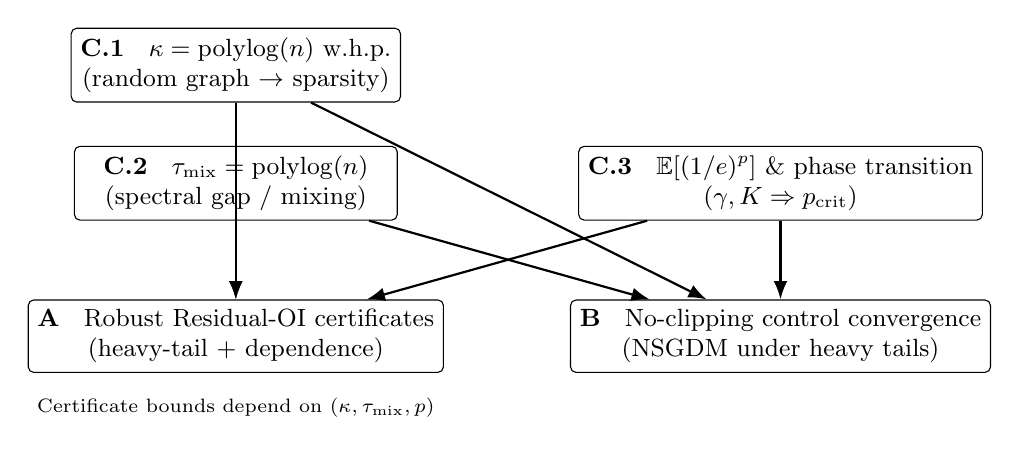
\begin{tikzpicture}[node distance=1.0em, every node/.style={font=\small}]
  \tikzstyle{n}=[draw,rounded corners=2pt,align=center,minimum width=4.1cm,minimum height=0.85cm]
  \tikzstyle{arrow}=[-Latex,thick]

  \node[n] (C1) {\textbf{C.1} \; $\kappa=\polylog(n)$ w.h.p.\\(random graph $\to$ sparsity)};
  \node[n,below=2.5cm of C1] (A) {\textbf{A} \; Robust Residual-OI certificates\\(heavy-tail + dependence)};
  \node[n,right=1.6cm of A] (B) {\textbf{B} \; No-clipping control convergence\\(NSGDM under heavy tails)};
  \node[n,above=1.0cm of B] (C3) {\textbf{C.3} \; $\E[(1/e)^p]$ \& phase transition\\($\gamma,K\Rightarrow p_{\mathrm{crit}}$)};
  \node[n,above=1.0cm of A] (C2) {\textbf{C.2} \; $\tau_{\mathrm{mix}}=\polylog(n)$\\(spectral gap / mixing)};

  \draw[arrow] (C1) -- (A);
  \draw[arrow] (C2) -- (A);
  \draw[arrow] (C3) -- (A);
  \draw[arrow] (C1) -- (B);
  \draw[arrow] (C2) -- (B);
  \draw[arrow] (C3) -- (B);

  \node[align=center,font=\scriptsize,below=0.2cm of A] {Certificate bounds depend on $(\kappa,\tau_{\mathrm{mix}},p)$};
\end{tikzpicture}
\end{frame}

% --------------------
% Practical next steps / timeline
% --------------------
\begin{frame}{Working plan}
\small
\begin{enumerate}
  \item Model(s) picking.
  \item Prove C.1 (local neighborhoods / induced interference sparsity) with clean statements.
  \item Use C.1 + mixing assumptions to finalize A's certificate bound with explicit $T_{\mathrm{eff}}$.
  \item Add C.3 phase transition to interpret heavy-tail index $p$.
  \item Optionally add B (NSGDM) as a second theorem section; or keep B as an outlook.
\end{enumerate}

I need help with the random-graph theorems (C.1/C.2/C.3) and sharper dependence-aware concentration tools.


\end{frame}

% --------------------
% Closing
% --------------------
\begin{frame}{Discussion}

COPF gives a principled fairness framework for performative evolving graphs.
This work would add a theory backbone that can be published independently:
\textbf{heavy-tailed} statistics + \textbf{dependent} graph data + \textbf{random-graph} foundations.



\end{frame}

% --------------------
% Backup slides
% --------------------


\end{document}
